\documentclass[14pt]{beamer} %Makes presentation
%\documentclass[handout]{beamer} %Makes Handouts

%\usepackage{bbding}
\usepackage{textpos}
%\usepackage{alltt}
%\usepackage{verbatim}
\usepackage{graphicx}
\usepackage{color}
%\usepackage{booktabs}
%\usepackage{tabularx}
%\usepackage{multirow}
%\usepackage{colortbl} %Table overlays

\usetheme{Singapore} %Gray with fade at top
\useoutertheme[subsection=false]{miniframes} %Supppress subsection in header
\useinnertheme{rectangles} %Itemize/Enumerate boxes
\usecolortheme{seagull} %Color theme
\usecolortheme{rose} %Inner color theme

\definecolor{light-gray}{gray}{0.75}
\definecolor{dark-gray}{gray}{0.55}
\setbeamercolor{item}{fg=light-gray}
\setbeamercolor{enumerate item}{fg=dark-gray}

\setbeamertemplate{navigation symbols}{}
%\setbeamertemplate{mini frames}[default]
%\setbeamercovered{dynamics}
\setbeamerfont*{title}{size=\Large,series=\bfseries}

%\setbeameroption{notes on second screen} %Dual-Screen Notes
%\setbeameroption{show only notes} %Notes Output

\setbeamertemplate{frametitle}{\vspace{.5em}\bfseries\insertframetitle}
\newcommand{\heading}[1]{\noindent \textbf{#1}\\ \vspace{1em}}

\newcommand\blfootnote[1]{%
  \begingroup
  \renewcommand\thefootnote{}\footnote{#1}%
  \addtocounter{footnote}{-1}%
  \endgroup
}

\newcommand{\blackslide}[1]{\bgroup
\setbeamercolor{background canvas}{bg=black}
\setbeamertemplate{navigation symbols}{}
\frame[plain]{\textcolor{white}{#1}}
\egroup}

%\usepackage{lmodern}
\usepackage{helvet}
\renewcommand{\familydefault}{\sfdefault}
\usepackage[english]{babel}
\usepackage[latin1]{inputenc}
\usepackage[T1]{fontenc}

\author[]{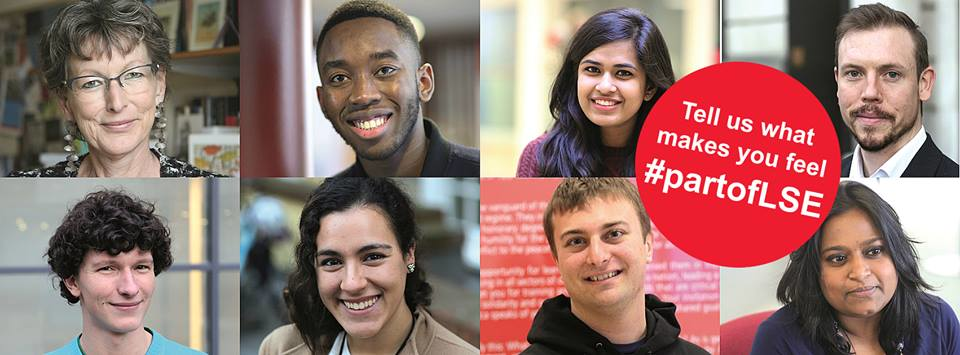
\includegraphics[width=.8\textwidth]{images/partoflse}}
\usepackage{tikz}
\usetikzlibrary{shapes,arrows}

\title{Government Department Subject Talk}

\date[]{29 March 2017}

\begin{document}

\frame{\titlepage}

% Hong Kong Theatre, Clement House
% 9.45-10.30am

% Self-introduction (5 minutes)
% Research-informed teaching (5 minutes)
% Substantive lecture (15 minutes)
% Time for Q&A (10 min)

% Welcome!


\frame[label=programmes]{

\frametitle{Degree programmes}

\begin{itemize}
\item BSc Government
\item BSc Government and Economics
\item BSc Government and History
\item BSc Politics and International Relations
\item BSc Politics and Philosophy

\vspace{1em}
\item PPE (administered by Philosophy)
\end{itemize}

}


\frame{
	\frametitle{Who am I?}
	\begin{itemize}\itemsep1em
    	\item Dr Thomas J. Leeper
    	\item Assistant Professor in Political Behaviour
    	\item PhD Political Science, 2012\\ Northwestern University
    	\item Undergraduate teaching
    		\begin{itemize}
    		\item ``Research Design in Political Science''
    		\item ``Experimental Politics''
    		\end{itemize}
	\end{itemize}
}

\frame{\tableofcontents}

\section{Why Government at LSE?}
\frame{\tableofcontents[currentsection]}


\blackslide{\centering\Large\textbf{Location, location, location\dots}}

\blackslide{\centering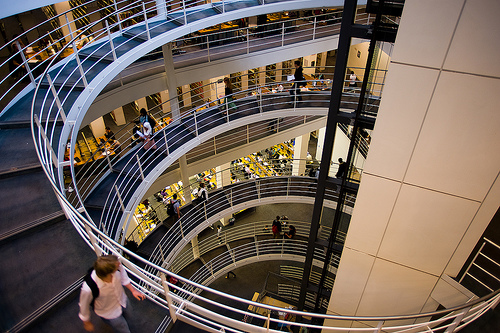
\includegraphics[width=\textwidth]{images/lse-library}}

\blackslide{\centering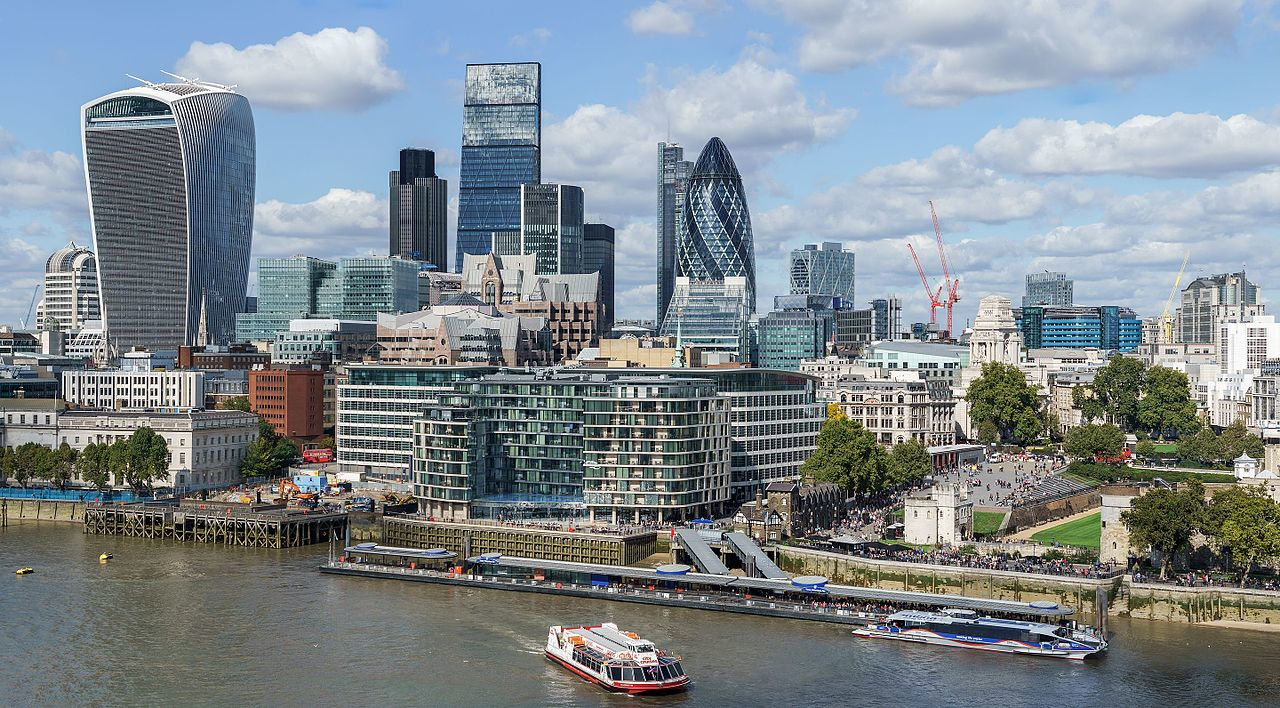
\includegraphics[width=\textwidth]{images/city-of-london}}

\blackslide{\centering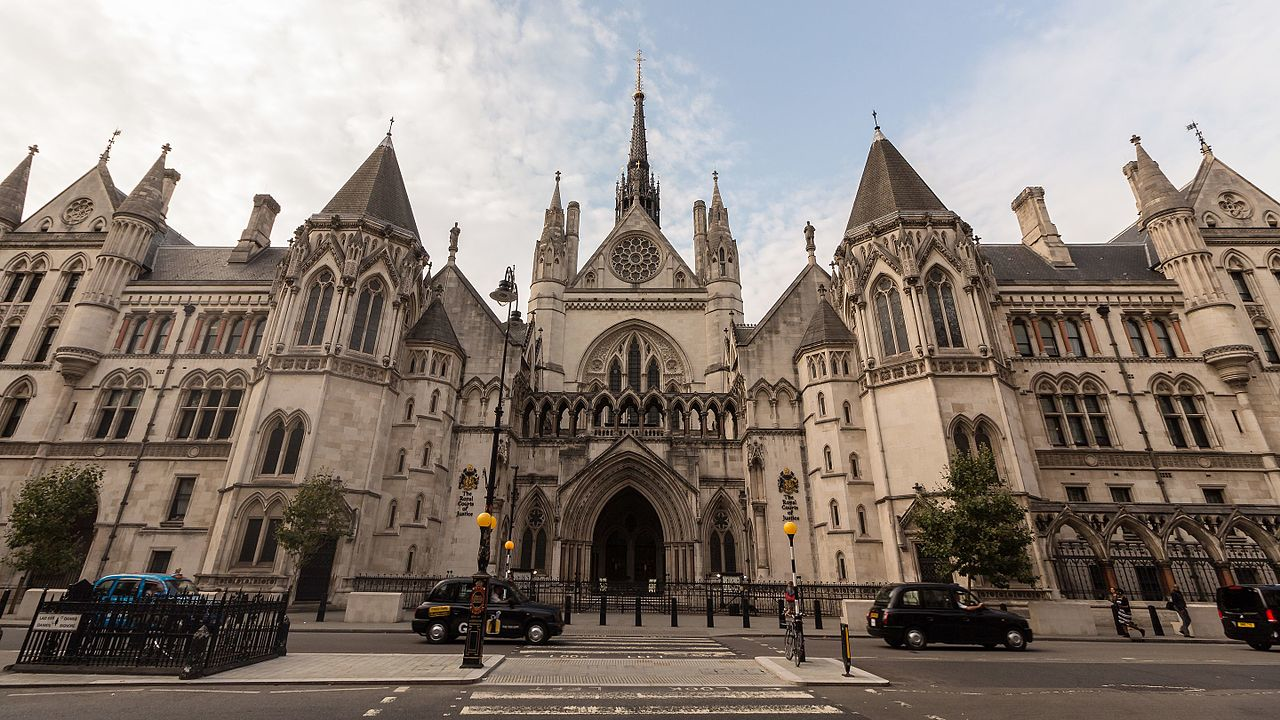
\includegraphics[width=\textwidth]{images/royal-courts}}

\blackslide{\centering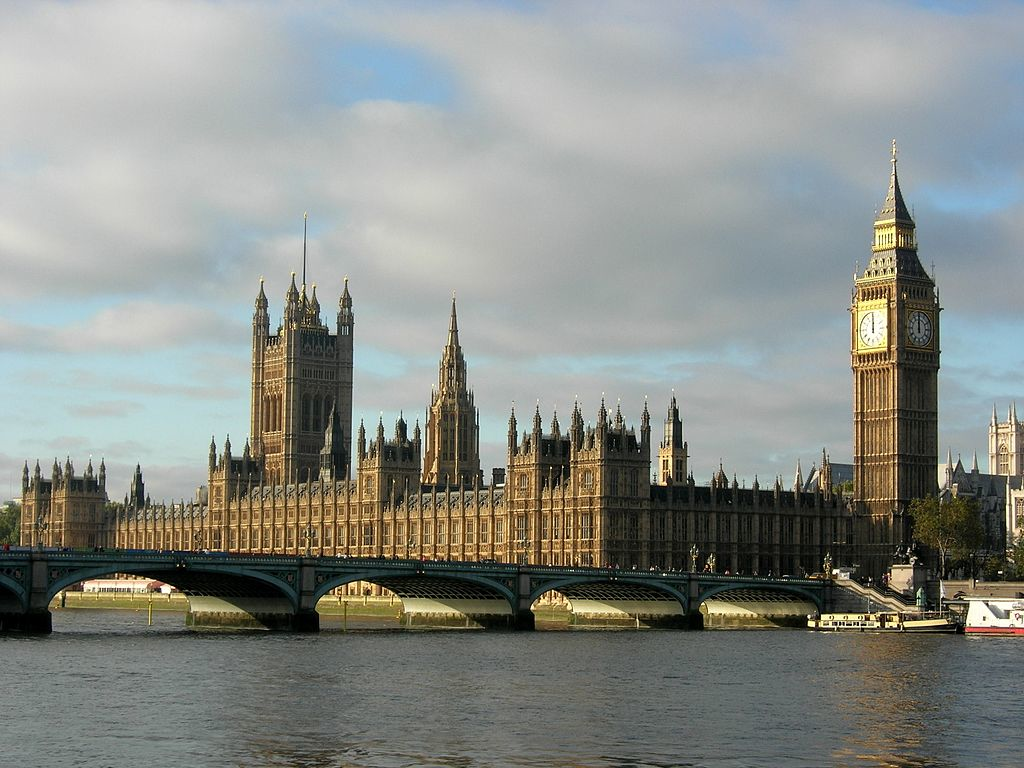
\includegraphics[width=\textwidth]{images/westminster}}

\blackslide{\centering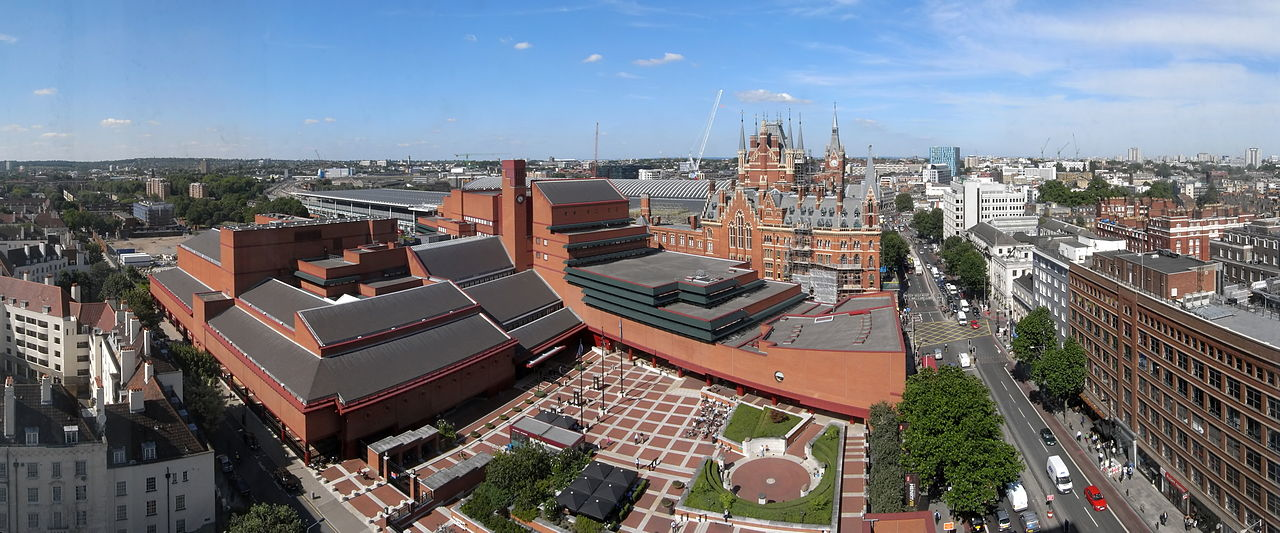
\includegraphics[width=\textwidth]{images/british-library}}

\blackslide{}

%On-campus resources - library
%Off-campus resources
%Hub of intellectual life in London
%Public events series

\blackslide{\centering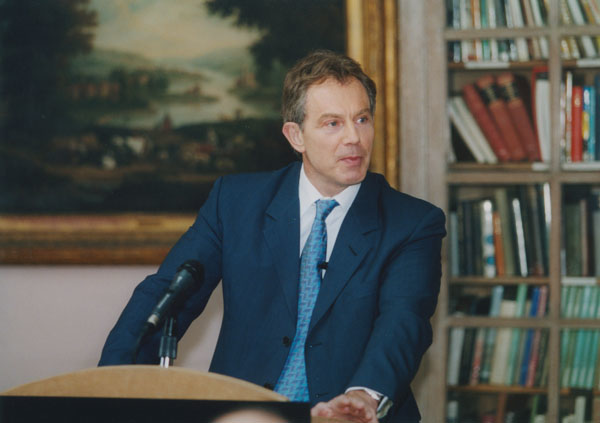
\includegraphics[width=\textwidth]{images/tony-blair}}

\blackslide{\centering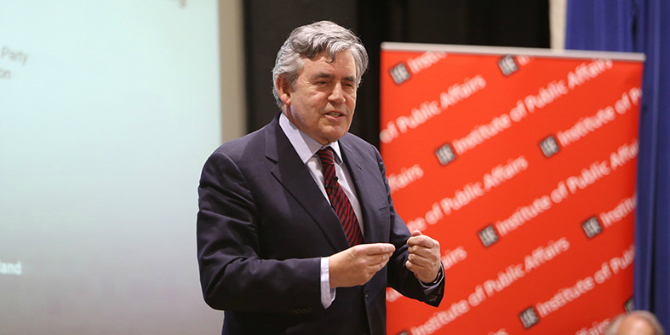
\includegraphics[width=\textwidth]{images/gordon-brown}}

\blackslide{\centering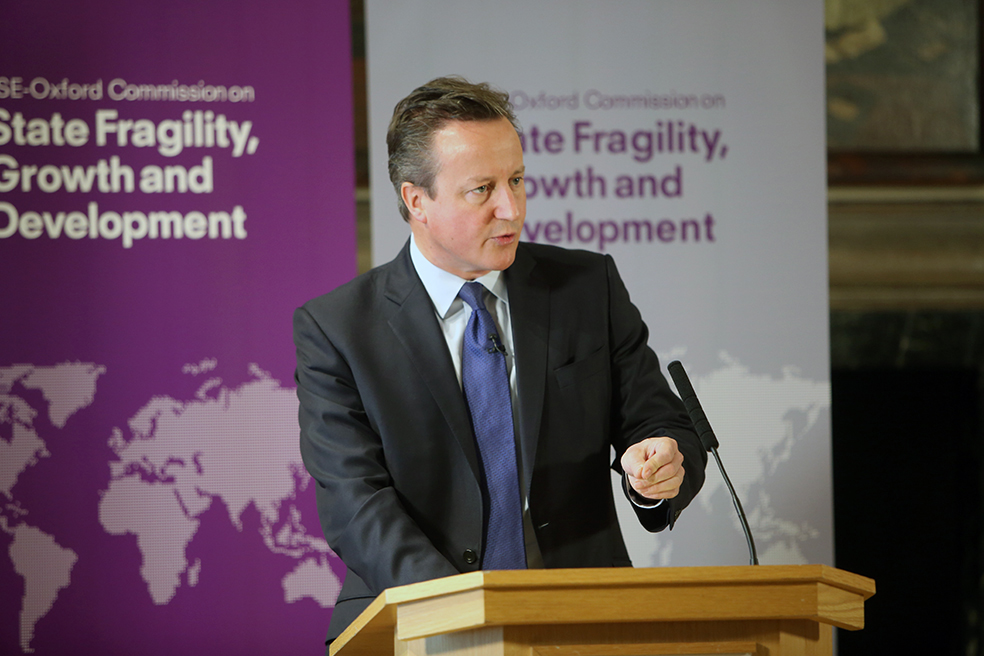
\includegraphics[width=\textwidth]{images/david-cameron}}

\blackslide{\centering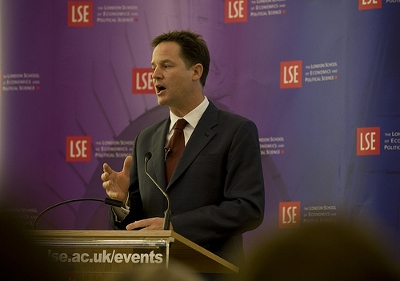
\includegraphics[width=\textwidth]{images/nick-clegg}}

\blackslide{\centering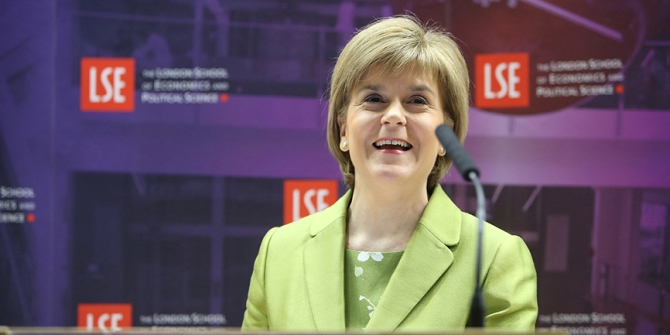
\includegraphics[width=\textwidth]{images/nicola-sturgeon}}

\blackslide{}


\blackslide{\centering\Large\textbf{Your fellow students\dots}}
%networking
% 5000 undergraduates, half of whom are from overseas (160 countries)
% 200+ student societies
% partnerships w/ Columbia Unviersity, Peking University, Science Po, University of Cape Town, and National University of Singapore

\blackslide{\centering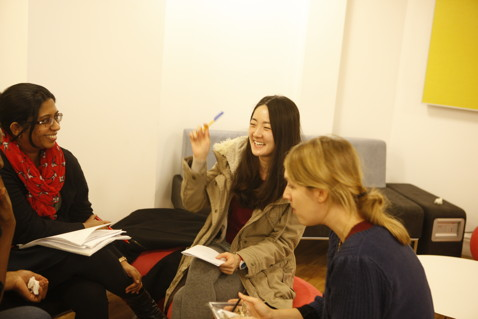
\includegraphics[width=\textwidth]{images/lif-8324}}

\blackslide{\centering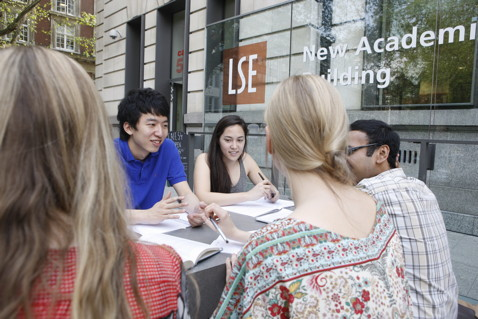
\includegraphics[width=\textwidth]{images/prospectus-9713}}

\blackslide{\centering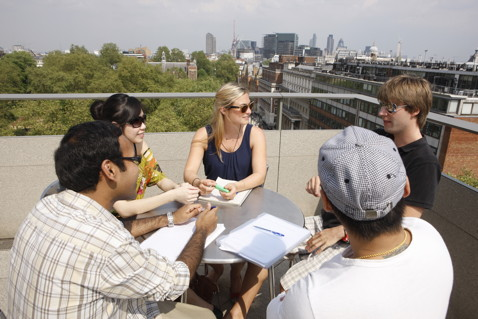
\includegraphics[width=\textwidth]{images/prospectus-9610}}

\blackslide{\centering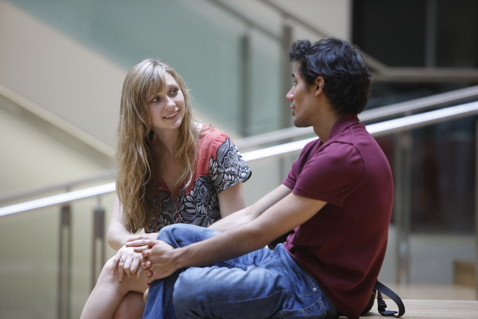
\includegraphics[width=\textwidth]{images/prospectus-9655}}

\blackslide{\centering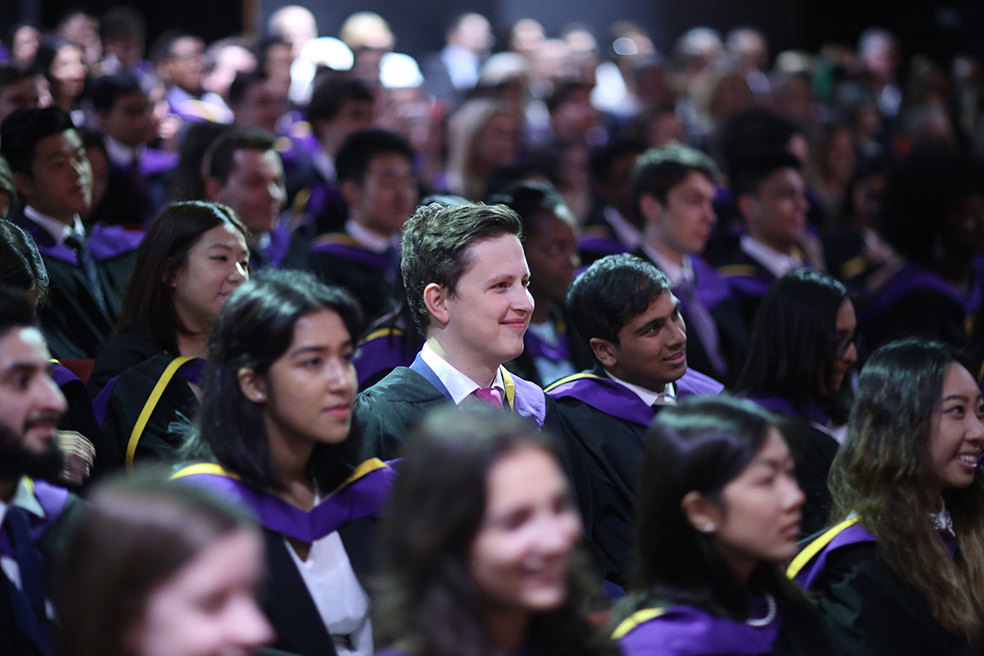
\includegraphics[width=\textwidth]{images/graduation-2016-1609}}

\blackslide{\centering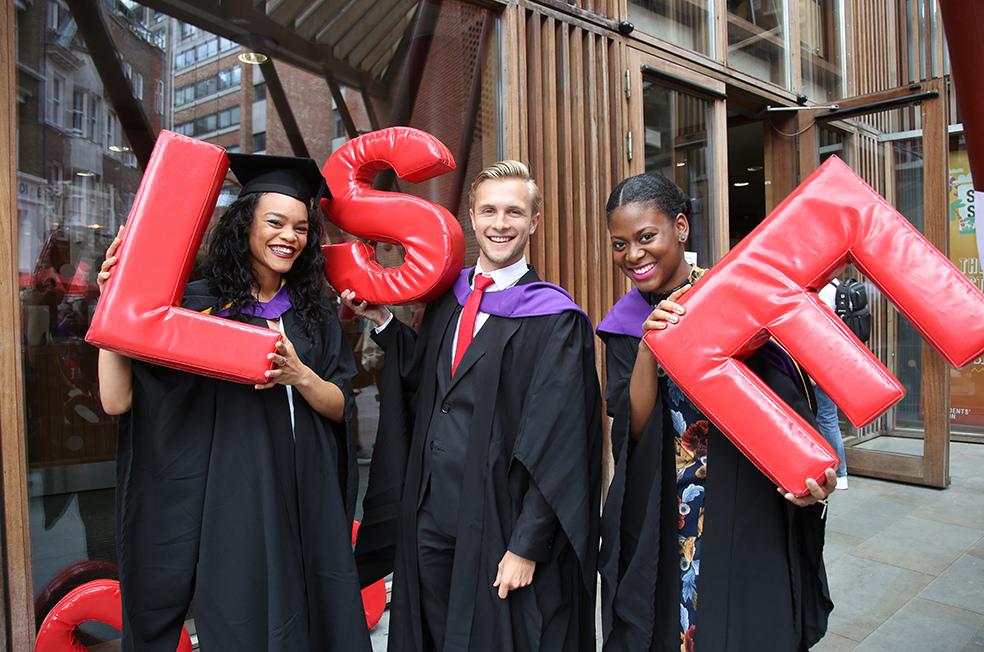
\includegraphics[width=\textwidth]{images/graduation-2016-1743}}

% ALUMNI:  Presidents or Prime Ministers of the UK, the US, Greece, Colombia, Taiwan, Japan, India, dozens of MPs and other politicians, 6 Nobel laureates; Thomas Piketty, Michael Oakeshott; Queen of Denmark, Mick Jagger, David Attenborough, and George Soros

\blackslide{}

\blackslide{\centering\Large\textbf{The academic staff\dots}}

%% most international academic staff in the UK
%% 2nd best places in the world to study social sciences
%% top REF (highest proportion of world-leading research in the whole of the UK)
%% media appearances, evidence at parliament

\blackslide{\centering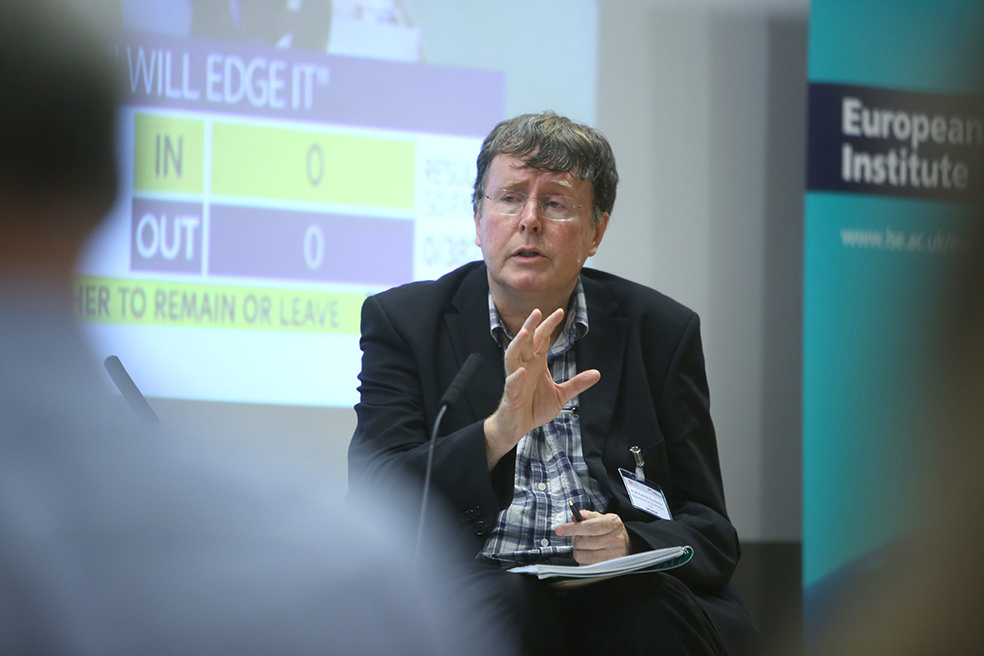
\includegraphics[width=\textwidth]{images/dunleavy-9769}}

\blackslide{\centering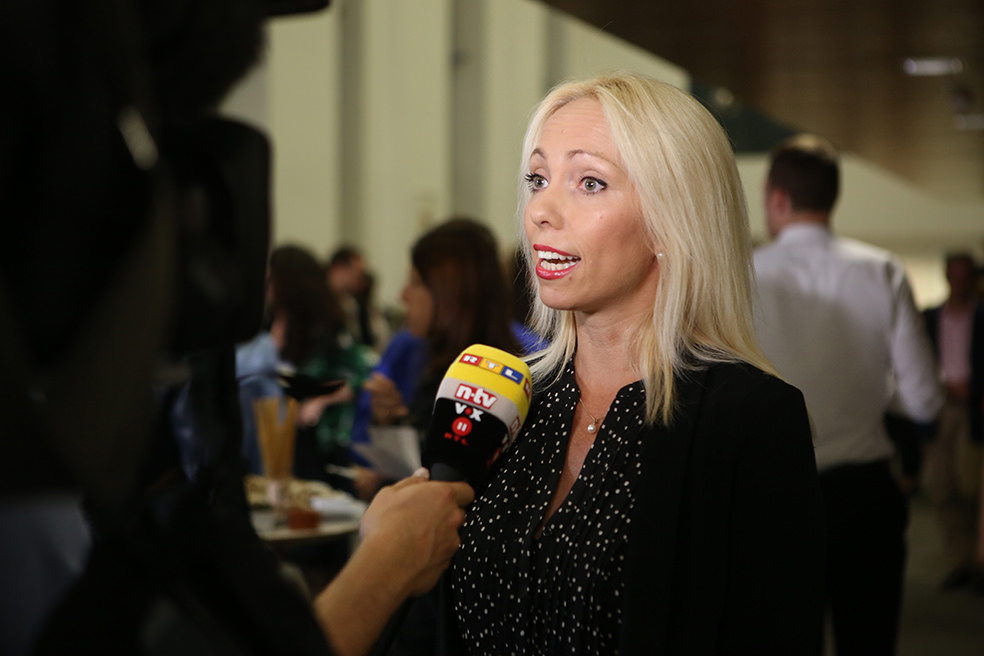
\includegraphics[width=\textwidth]{images/hobolt-9369}}

\blackslide{\centering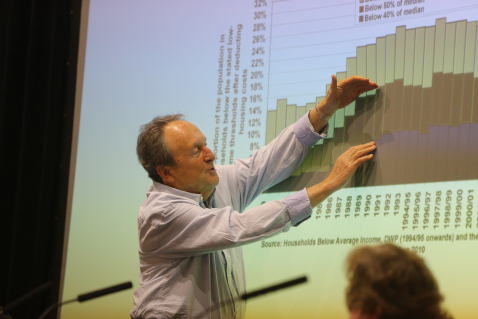
\includegraphics[width=\textwidth]{images/soskice-7292}}

\blackslide{}

% Research-Informed Teaching
\section[Research-informed Teaching]{What Is Research-informed Teaching?}
%\frame{\tableofcontents[currentsection]}

\blackslide{\centering\Large\textbf{Research-informed teaching\dots}\blfootnote{\textcolor{white}{\url{https://www.lse.ac.uk/About-LSE/Our-strategy}}}
}

\blackslide{\centering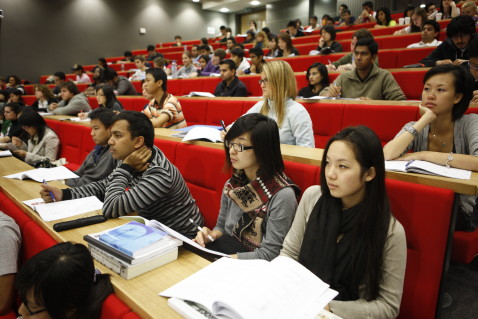
\includegraphics[width=\textwidth]{images/nab-9852}}

\blackslide{\centering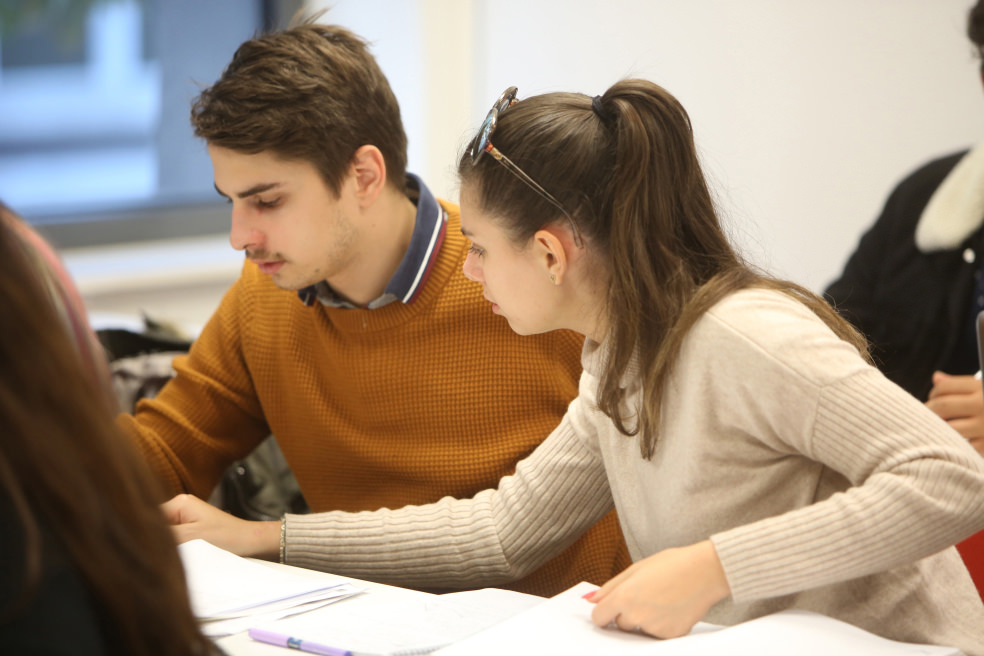
\includegraphics[width=\textwidth]{images/teaching-5940}}

\blackslide{\centering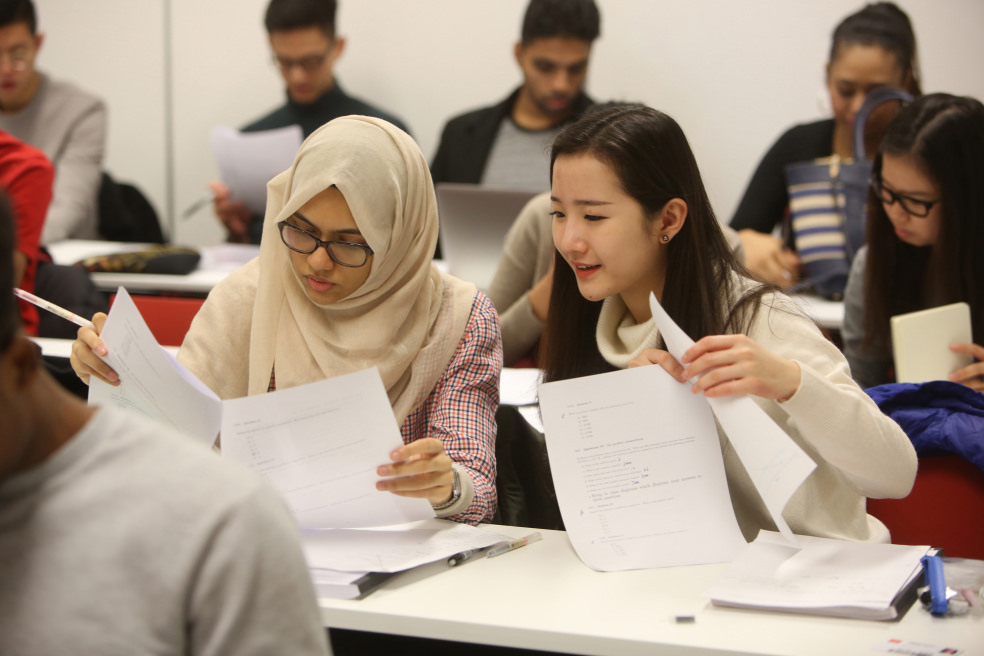
\includegraphics[width=\textwidth]{images/teaching-5938}}

\blackslide{\centering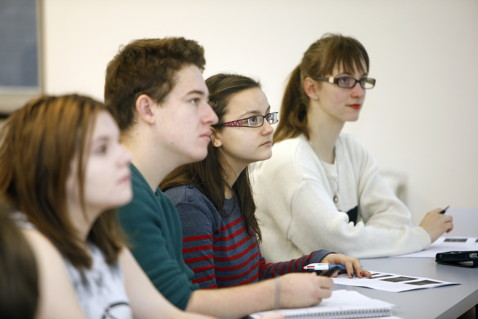
\includegraphics[width=\textwidth]{images/teaching-7055}}

{
\usebackgroundtemplate{
\includegraphics[height=\paperheight,width=\paperwidth]{images/education-strategy-image}}
\begin{frame}[plain]
\end{frame}
}
    


\frame{

\frametitle{Features of an LSE Education}

\begin{enumerate}\itemsep0.5em
\item One-on-one advising from member of academic staff
\item<2-> Small and large group teaching
\item<3-> LSE100: The LSE Course
\item<4-> Undergraduate research opportunities
	\begin{itemize}
	\item Coursework
	\item Undergraduate research internships
	\item LSE Groups
	\item Posters in Parliament
	\item Research seminar series
	\end{itemize}
\item<5-> Dissertation
\end{enumerate}

}


\frame{

\frametitle{General Course Structure}

\begin{enumerate}\itemsep1em
\item First Year
	\begin{itemize}
	\item ``Introduction to Political Science''
	\item ``Introduction to Political Theory''
	\item Two further modules
	\item LSE100
	\end{itemize}
\item<2-> Second Year
	\begin{itemize}
	\item Mix of Government and other modules
	\item Expand breadth of knowledge
	\end{itemize}
\item<3-> Third Year
	\begin{itemize}
	\item Advanced seminars ($n<15$)
	\item Optional dissertation
	\end{itemize}
\end{enumerate}

}

\againframe{programmes}

% causal inference


\blackslide{}

\blackslide{\vspace{4em}\begin{center}\Large\textbf{``Rerum cognoscere causas''}\\\vspace{2em}\onslide<2->{\textit{To know the causes of things}}\end{center}}



\frame[label=types]{
	\frametitle{{\large ``Rerum cognoscere causas''}}
	\begin{itemize}\itemsep1.5em
		\item Forward causal questions
			\begin{itemize}\itemsep0.5em
    			\item<2-> What effect(s) does X have?
    			\item<3-> ``What if?'' questions
			\end{itemize}
		\item Backward causal questions
			\begin{itemize}
    			\item<4-> What causes Y?
    			\item<5-> Why does Y occur?
			\end{itemize}
	\end{itemize}
}


% forward

\blackslide{\Large\centering\textbf{What effect did the end of South Africa apartheid have public goods delivery?}}

\blackslide{\Large\centering\textbf{What role do gender quotas have on the political participation of women?}}

\blackslide{\Large\centering\textbf{How can governments use liberal-paternalist \textit{nudges} to affect public behaviour?}}

\blackslide{\Large\centering\textbf{What effect will Britain's exit from the EU have on British economic and social life?}}

\blackslide{\Large\centering\textbf{How do land rights shape the political behaviour and institutions of Sub-Saharan Africa?}}

\blackslide{\Large\centering\textbf{How do elections affect citizens emotionally?}}

\blackslide{\Large\centering\textbf{What effect did protest activity have during the Arab Spring?}}

\blackslide{\Large\centering\textbf{How does the non-verbal behaviour of Bank of England Governors affect their political influence?}}

\blackslide{\Large\centering\textbf{How do immigration policies affect the political and economic freedoms of the native-born?}}

\blackslide{}

% backward

\blackslide{\Large\centering\textbf{Why did some people vote to Leave the EU while others voted to Remain?}}

\blackslide{\Large\centering\textbf{How does nationalism develop in the politics of South-East Asian states?}}

\blackslide{\Large\centering\textbf{How do local politicians make decisions about aid distribution in Malawi?}}

\blackslide{\Large\centering\textbf{Why do so many terrorists have degrees in engineering?}}

\blackslide{\Large\centering\textbf{How do leaders of one-party states decide which partisans to purge to preserve political control?}}

\blackslide{\Large\centering\textbf{How do post-conflict societies build stable political institutions?}}

\blackslide{}

\frame<1-2>[label=whatworks]{

\frametitle{``What works?'' discourse}

\begin{itemize}\itemsep1.5em
\item Causal inference is not just an academic exercise

\item<2-> Governments, firms, and NGOs worldwide want to know \textit{what works?}

\item<3-> To do that we need students to not just be passionate about learning what we already know but also \textit{creating} new knowledge
\end{itemize}

}


\blackslide{\centering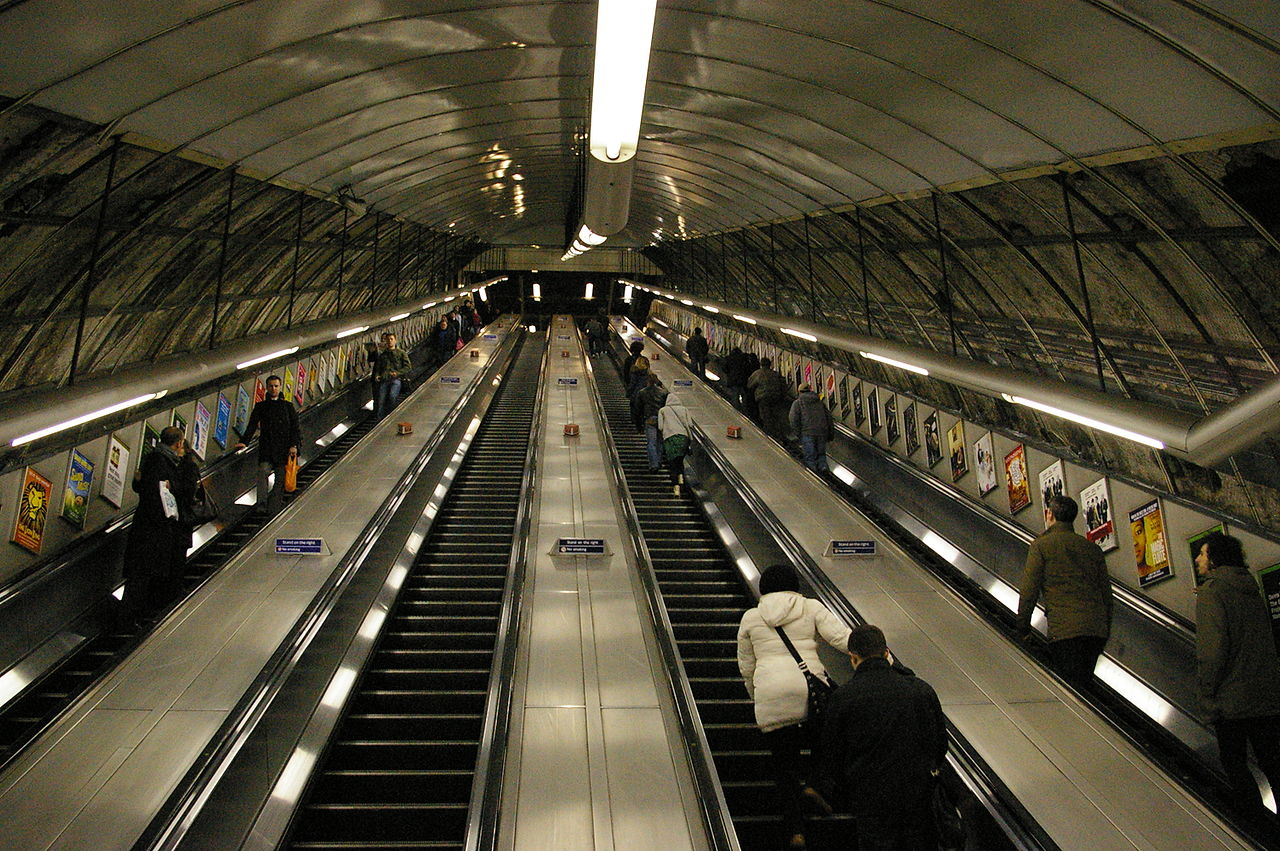
\includegraphics[width=\textwidth]{images/holborn}}


\againframe<2-3>{whatworks}

\frame{

\frametitle{Drawing causal inferences}

\begin{itemize}\itemsep1.5em
\item<1-> Causal inference is the effort to \textit{explain} how and why the world works as it does\\
	\begin{itemize}\itemsep0.5em
	\item What consequences does \textit{something} have?
	\item Why does \textit{something} happen?
	\end{itemize}
\item<2-> This goes beyond looking for patterns\\
	\begin{itemize}
	\item Correlation is not correlation!
	\end{itemize}
\item<3-> How, then, do we identify causal relationships in politics?
\end{itemize}

}

% Methodology: ``tools for gathering and analyzing data to try to make valid inferences''


\frame{
\frametitle{Fundamental problem of causal inference}

\large

Causal inference involves inferring \textit{what would have happened} in a counterfactual reality \textit{where the potential cause took on a different value}\\

\vspace{2em}

\only<2->{We can only observe the reality that occurs!}

}

\frame{
\frametitle{``A Christmas Carol''}

\small 
\begin{itemize}
\item 1843 novel by Charles Dickens
\item Ebenezer Scrooge is shown his own future by the ``Ghost of Christmas Yet to Come''
\item Has the choice to either:
	\begin{itemize}
	\item stay on current path (one counterfactual), or 
	\item change his ways (take a different counterfactual)
	\end{itemize}
\end{itemize}
}


% Groundhog Day
% 13 Going On 30
% Run Lola Run
% Source Code
% X-Mean: Days of Future Past


\frame{
\frametitle{Drawing causal inferences}

\begin{itemize}\itemsep1.5em
\item Causality is defined as the difference between two \textit{potential} outcomes:\\
	\begin{enumerate}\itemsep0.5em
	\item the outcome that occurs if $X$ occurs
	\item the outcome that occurs if $X$ does not occur
	\end{enumerate}
\item<2-> To \textit{know the causes of things} we need to know how to gather evidence and process that evidence in order to \textit{infer} causality when we cannot see it directly
\end{itemize}

}


\frame[plain]{}

\frame[plain]{
\vspace{2em}
\begin{center}
\Large
\includegraphics[width=.5\textheight]{images/lse-beaver}\\\vspace{1em}\onslide<2->{\textit{What works?}}
\end{center}
}


\section{Q \& A}
%\frame{\tableofcontents[currentsection]}

\frame{

For more information\dots

\small

\begin{itemize}\itemsep0.5em
\item \dots about admissions:\\
``Applying to LSE'' (Old Theatre): 11:30, 12:30, 14:30

\item \dots about courses:\\
\url{http://www.lse.ac.uk/resources/calendar/Default.htm}

\item \dots about the Government Department:\\
\url{http://www.lse.ac.uk/government/home.aspx}

\item \dots about LSE Education Strategy:\\
\url{https://www.lse.ac.uk/about-lse/Image-assets/PDF/Education-Strategy.pdf}

\item \dots about public events:\\
\url{http://www.lse.ac.uk/Events}
\end{itemize}
}

\frame{\vspace{4em}\Huge\centering \textbf{Questions?}}

\blackslide{}


\appendix

\frame{

\small
Photo credits

\tiny

\begin{itemize}
\item \url{https://commons.wikimedia.org/wiki/File:City_of_London_skyline_from_London_City_Hall_-_Sept_2015_-_Crop_Aligned.jpg}

\item \url{https://commons.wikimedia.org/wiki/File:Palacio_de_Westminster_-_panoramio.jpg}

\item \url{https://commons.wikimedia.org/wiki/File:Royal_Courts_of_Justice_-_Wide_Angle_Front.jpg}

\item \url{https://commons.wikimedia.org/wiki/File:Lselibray_2.jpg}

\item \url{http://blogs.lse.ac.uk/communications/files/2015/09/Facebook-pic-2-1024x538.jpg}

\item \url{https://commons.wikimedia.org/wiki/File:British_Library_\%2B_St_Pancras_7527-31hug.jpg}

\item \url{https://www.flickr.com/photos/lselibrary/22737505912/in/album-72157658449873093/}

\item \url{https://www.flickr.com/photos/lselibrary/22737505912/in/album-72157658449873093/}

\item \url{http://blogs.lse.ac.uk/politicsandpolicy/files/2011/09/Nick-Clegg-LSE.jpg}

\item \url{http://blogs.lse.ac.uk/politicsandpolicy/reevaluating-gordon-brown-its-important-to-factor-context-into-our-assessment-of-political-leaders/}

\item \url{https://www.flickr.com/photos/lselibrary/4153090140}

\item \url{http://www.ox.ac.uk/sites/files/oxford/styles/ow_medium_feature/public/field/field_image_main/Cameron\%20DSC05394_0.JPG?itok=JwW75lKI}

\item \url{http://blogs.lse.ac.uk/politicsandpolicy/five-minutes-with-nicola-sturgeon-minority-government-is-perfectly-capable-of-being-stable-government/}

\end{itemize}

}

\blackslide{}

\end{document}

